\documentclass[11pt,a4paper]{article}
\usepackage{fontspec}
\setmainfont{TeX Gyre Pagella}
\setmonofont{Inconsolatazi4}

\usepackage{tikz}
\usetikzlibrary{positioning, arrows.meta, fit, backgrounds, calc}

\usepackage{amsmath, amssymb}
\usepackage{booktabs}
\usepackage{enumitem}
\usepackage[margin=2.5cm]{geometry}
\usepackage{xcolor}
\usepackage{listings}

\definecolor{corecordblue}{RGB}{40, 80, 160}
\definecolor{pyobjgreen}{RGB}{40, 130, 60}
\definecolor{disciplineorange}{RGB}{200, 100, 20}
\definecolor{dualred}{RGB}{180, 40, 40}
\definecolor{codebg}{RGB}{248, 248, 248}

\lstset{
  basicstyle=\ttfamily\small,
  backgroundcolor=\color{codebg},
  frame=single,
  framerule=0.4pt,
  rulecolor=\color{black!20},
  columns=fullflexible,
  keepspaces=true,
  breaklines=true,
}

\title{\textbf{Corecord Unification}\\[0.3em]
\large ANFJoin as Universal IR Construction}
\author{Carter Schonwald}
\date{March 2026}

\begin{document}
\maketitle

\section{The Observation}

\texttt{ANFJoin} is not specific to control flow merge points. It is
the universal construction for everything the IR \emph{builds}---any
entity defined by its observations (methods/fields) over a shared
closure.

Join points, generators, objects, iterators, and context managers
are the same codata construction with different \textbf{usage
disciplines}.

\section{The Corecord}

A corecord (coinductive record) is defined by:
\begin{itemize}[nosep]
  \item A set of named \textbf{fields} (observations/methods)
  \item A \textbf{shared closure} $\Gamma$ (the additive \& property)
  \item Each field has its own type signature and body
\end{itemize}

\begin{lstlisting}
corecord C over {shared_env} =
  | .field_1(params_1) -> body_1
  | .field_2(params_2) -> body_2
  | ...
\end{lstlisting}

Elimination is observation: $c.\mathsf{field}_k(\mathit{args})$.
Construction is copattern matching.

\section{Usage Discipline Spectrum}

\begin{center}
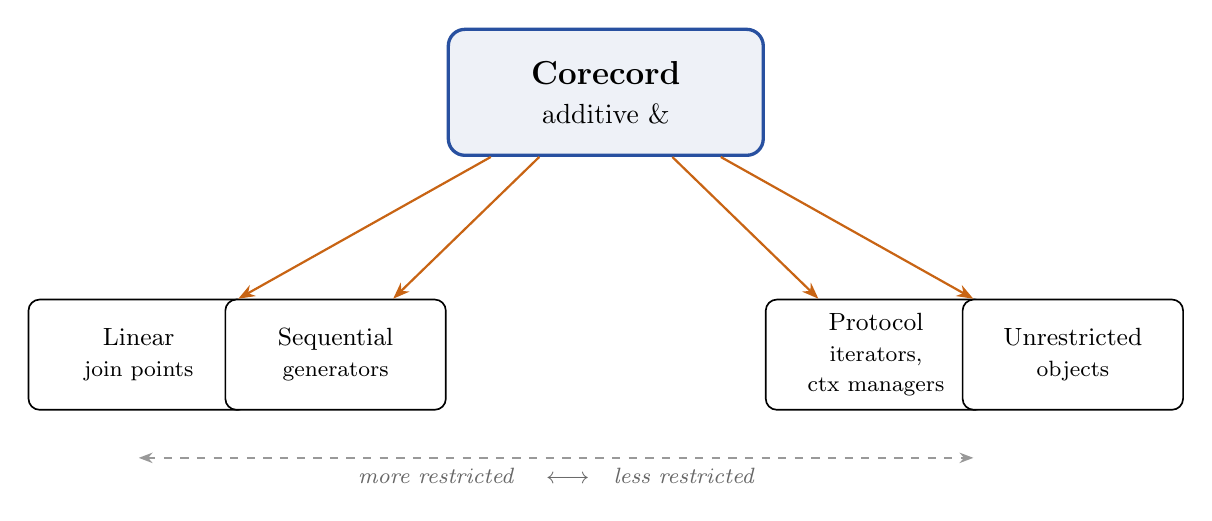
\begin{tikzpicture}[
    discipline/.style={
      draw, rounded corners=4pt, minimum width=2.8cm,
      minimum height=1.4cm, align=center, font=\small,
      fill=white, line width=0.6pt
    },
    corecbox/.style={
      draw=corecordblue, rounded corners=6pt, minimum width=4cm,
      minimum height=1.6cm, align=center, font=\large\bfseries,
      fill=corecordblue!8, line width=1.2pt
    },
    arrow/.style={-{Stealth[length=6pt]}, thick, disciplineorange},
    label/.style={font=\footnotesize\itshape, disciplineorange},
    node distance=1.2cm and 1.5cm,
]
    % Corecord at top
    \node[corecbox] (corec) {Corecord\\{\normalsize\normalfont additive \&}};

    % Usage disciplines below
    \node[discipline, below left=1.8cm and 2.5cm of corec] (linear)
      {Linear\\{\footnotesize join points}};
    \node[discipline, below left=1.8cm and 0cm of corec] (seq)
      {Sequential\\{\footnotesize generators}};
    \node[discipline, below right=1.8cm and 0cm of corec] (proto)
      {Protocol\\{\footnotesize iterators,}\\{\footnotesize ctx managers}};
    \node[discipline, below right=1.8cm and 2.5cm of corec] (unres)
      {Unrestricted\\{\footnotesize objects}};

    % Arrows from corecord
    \draw[arrow] (corec) -- (linear);
    \draw[arrow] (corec) -- (seq);
    \draw[arrow] (corec) -- (proto);
    \draw[arrow] (corec) -- (unres);

    % Spectrum arrow at bottom
    \draw[{Stealth[length=5pt]}-{Stealth[length=5pt]},
          thick, black!40, dashed]
      (linear.south) ++(0,-0.6) -- ++(10.6,0)
      node[midway, below, font=\footnotesize\itshape, black!60]
      {more restricted \quad$\longleftrightarrow$\quad less restricted};
\end{tikzpicture}
\end{center}

All four are the \emph{same} \&-typed corecord over a shared closure.
The axis is how many fields may be observed and in what order.

\begin{table}[h]
\centering
\begin{tabular}{@{}llll@{}}
\toprule
\textbf{Discipline} & \textbf{Fields called} & \textbf{Enforcement} & \textbf{Python example} \\
\midrule
Linear       & exactly one, once  & compiler (CFG)   & \texttt{if/else} merge \\
Sequential   & in order, once each & runtime protocol & generators \\
Protocol     & specified order    & convention/types  & context managers \\
Unrestricted & any, any order     & none             & objects \\
\bottomrule
\end{tabular}
\end{table}

\section{Two-Layer Architecture}

\begin{center}
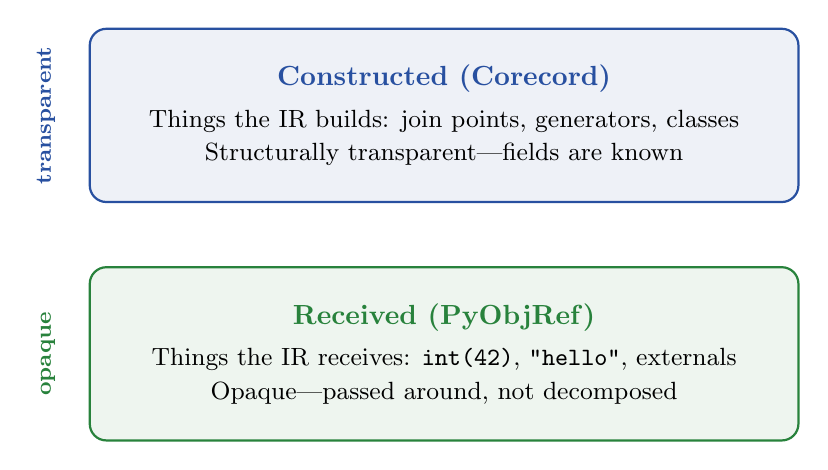
\begin{tikzpicture}[
    layer/.style={
      draw, rounded corners=6pt, minimum width=9cm,
      minimum height=2.2cm, align=center, line width=0.8pt
    },
    node distance=0.8cm,
]
    \node[layer, fill=corecordblue!8, draw=corecordblue] (constructed)
      {\textbf{\color{corecordblue}Constructed (Corecord)}\\[3pt]
       \small Things the IR builds: join points, generators, classes\\
       \small Structurally transparent---fields are known};

    \node[layer, fill=pyobjgreen!8, draw=pyobjgreen, below=of constructed] (received)
      {\textbf{\color{pyobjgreen}Received (PyObjRef)}\\[3pt]
       \small Things the IR receives: \texttt{int(42)}, \texttt{"hello"}, externals\\
       \small Opaque---passed around, not decomposed};

    % Labels
    \node[left=0.3cm of constructed, font=\footnotesize\bfseries,
          corecordblue, rotate=90, anchor=south] {transparent};
    \node[left=0.3cm of received, font=\footnotesize\bfseries,
          pyobjgreen, rotate=90, anchor=south] {opaque};
\end{tikzpicture}
\end{center}

These are complementary. A \texttt{def} in analyzed source produces a
corecord. An \texttt{int(42)} produces a PyObjRef. The PyDatum cleanup
(closed types for embeddable literals) is orthogonal.

\section{Instantiations}

\subsection{Join Points (Linear)}

\begin{lstlisting}
join j over {a, b} =
  | .from_B0(x:int, y:int) -> body(a, b, x, y)
  | .from_B1(x:str, y:int) -> body(a, b, x, y)

if cond then j.from_B0(1, 2)
         else j.from_B1("hi", 4)
\end{lstlisting}

Exactly one field invoked. Used once, immediately, internally.

\subsection{Generators (Sequential)}

\begin{lstlisting}
corecord gen over {frame_locals} =
  | .entry(args)     -> body_0 ... yield v_1 -> .resume_1
  | .resume_1(sent)  -> body_1 ... yield v_2 -> .resume_2
  | .resume_2(sent)  -> body_2 ... return final
\end{lstlisting}

\texttt{RETURN\_GENERATOR} marks construction as reified.
\texttt{YIELD\_VALUE} emits a field boundary.
\texttt{next(gen)} = \texttt{g.resume\_k(None)}.
No multi-entry CFG needed.

\subsection{Objects (Unrestricted)}

\begin{lstlisting}
corecord obj over {self.__dict__} =
  | .method_a(args) -> body_a
  | .method_b(args) -> body_b
  | .__getattr__(name) -> ...
\end{lstlisting}

\texttt{\_\_dict\_\_} is the shared closure.
Method call = field observation.

\section{AD Duality}

Under the dagger functor ($\dagger$), additive \& dualizes to
additive $\oplus$:

\begin{center}
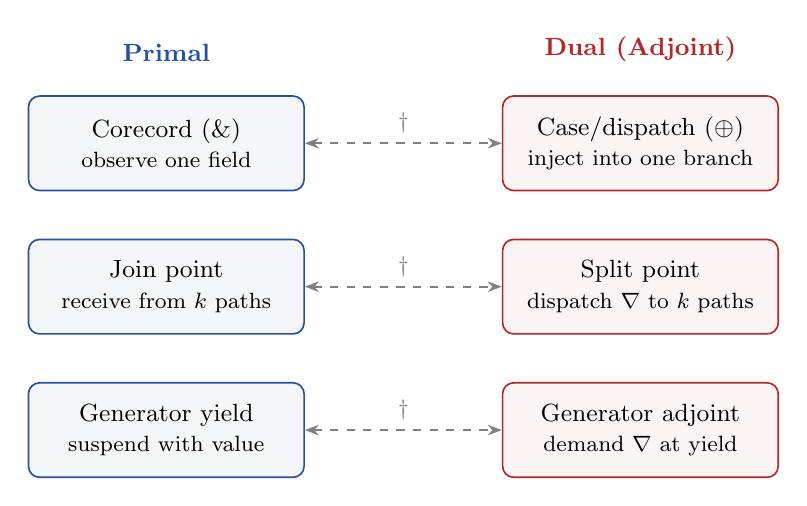
\begin{tikzpicture}[
    box/.style={
      draw, rounded corners=4pt, minimum width=3.5cm,
      minimum height=1.2cm, align=center, font=\small,
      line width=0.6pt
    },
    dualbox/.style={box, draw=dualred, fill=dualred!5},
    primalbox/.style={box, draw=corecordblue, fill=corecordblue!5},
    dualarrow/.style={
      {Stealth[length=5pt]}-{Stealth[length=5pt]},
      thick, black!50, dashed
    },
    node distance=0.6cm and 2.5cm,
]
    % Primal column
    \node[primalbox] (p1) {Corecord (\&)\\{\footnotesize observe one field}};
    \node[primalbox, below=of p1] (p2) {Join point\\{\footnotesize receive from $k$ paths}};
    \node[primalbox, below=of p2] (p3) {Generator yield\\{\footnotesize suspend with value}};

    % Dual column
    \node[dualbox, right=2.5cm of p1] (d1) {Case/dispatch ($\oplus$)\\{\footnotesize inject into one branch}};
    \node[dualbox, right=2.5cm of p2] (d2) {Split point\\{\footnotesize dispatch $\nabla$ to $k$ paths}};
    \node[dualbox, right=2.5cm of p3] (d3) {Generator adjoint\\{\footnotesize demand $\nabla$ at yield}};

    % Duality arrows
    \draw[dualarrow] (p1) -- node[above, font=\footnotesize] {$\dagger$} (d1);
    \draw[dualarrow] (p2) -- node[above, font=\footnotesize] {$\dagger$} (d2);
    \draw[dualarrow] (p3) -- node[above, font=\footnotesize] {$\dagger$} (d3);

    % Labels
    \node[above=0.3cm of p1, font=\small\bfseries, corecordblue] {Primal};
    \node[above=0.3cm of d1, font=\small\bfseries, dualred] {Dual (Adjoint)};
\end{tikzpicture}
\end{center}

Combined with multiplicative duality ($\mathrm{dup}^\dagger = \Sigma$
gradients, $\mathrm{drop}^\dagger = 0$), this gives complete mechanical
AD derivation from ANF + corecord structure.

\section{Literature}

\begin{table}[h]
\centering
\small
\begin{tabular}{@{}lll@{}}
\toprule
\textbf{Tradition} & \textbf{Name for this} & \textbf{Key reference} \\
\midrule
Linear logic   & Additive \& (with), $n$-ary & Girard (1987) \\
CBPV           & Negative type             & Levy (2004) \\
Agda           & Copattern matching        & Abel et al.\ (2013) \\
Agda OO        & Server-side programs ($\Pi\Sigma$) & Abel, Adelsberger \& Setzer (2016) \\
GHC Core       & Join points               & Peyton Jones et al.\ (2017) \\
$\Pi$--$\Sigma$ & \& from the type former  & Schonwald (2026) \\
Polarity       & Negative, focusing        & Zeilberger (2009) \\
\bottomrule
\end{tabular}
\end{table}

The ooAgda paper (Abel, Adelsberger \& Setzer 2016) develops exactly
this idea---objects as server-side interactive programs via
copatterns---but in the context of dependently-typed
\emph{programming}. 15 citations in 10 years (Semantic Scholar, March
2026); the insight did not propagate into compiler IR design. We apply
it to a bytecode IR for Python.

\section{Termination}

Three termination arguments, one per traversal mode.

\subsection{Code Object Traversal}

Code objects form a \textbf{finite DAG} via \texttt{co\_consts}. Inner
functions, classes, comprehensions, and generators appear as code
objects in their enclosing function's \texttt{co\_consts} tuple. Inner
code objects do not reference their parent. Recursive descent is
structural recursion on a strict substructure.

\subsection{Abstract Interpretation}

Bounded by: finite-height lattice $\times$ finite CFG.
$O(|\text{blocks}| \times h)$ where $h$ is lattice height.
Widening handles infinite-height lattices.

\subsection{The Static Visibility Boundary}

The IR can see inside a code object iff it appears in the static
\texttt{co\_consts} DAG. This is the corecord/PyObjRef boundary:

\begin{center}
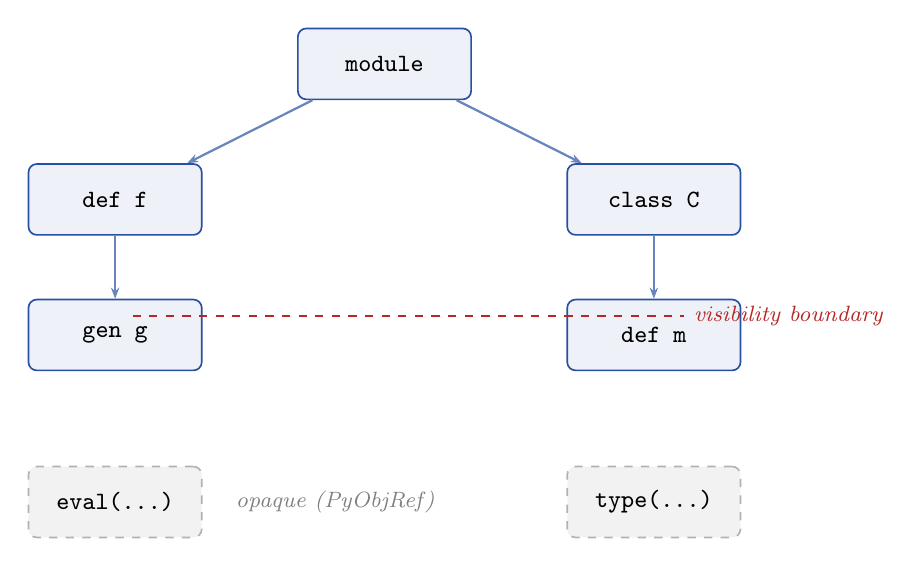
\begin{tikzpicture}[
    dag/.style={
      draw, rounded corners=3pt, minimum width=2.2cm,
      minimum height=0.9cm, align=center, font=\small,
      fill=corecordblue!8, draw=corecordblue, line width=0.6pt
    },
    opaque/.style={
      draw, rounded corners=3pt, minimum width=2.2cm,
      minimum height=0.9cm, align=center, font=\small,
      fill=black!5, draw=black!30, line width=0.6pt, dashed
    },
    edge/.style={-{Stealth[length=4pt]}, thick, corecordblue!70},
    boundary/.style={thick, dashed, dualred},
    node distance=0.8cm and 1.2cm,
]
    % Static DAG
    \node[dag] (top) {\texttt{module}};
    \node[dag, below left=of top] (fn) {\texttt{def f}};
    \node[dag, below right=of top] (cls) {\texttt{class C}};
    \node[dag, below=of fn] (gen) {\texttt{gen g}};
    \node[dag, below=of cls] (meth) {\texttt{def m}};

    \draw[edge] (top) -- (fn);
    \draw[edge] (top) -- (cls);
    \draw[edge] (fn) -- (gen);
    \draw[edge] (cls) -- (meth);

    % Boundary
    \draw[boundary] (-3.2, -3.2) -- (3.8, -3.2)
      node[right, font=\footnotesize\itshape, dualred] {visibility boundary};

    % Opaque
    \node[opaque, below=1.2cm of gen] (eval) {\texttt{eval(...)}};
    \node[opaque, below=1.2cm of meth] (dyn) {\texttt{type(...)}};

    \node[right=0.3cm of eval, font=\footnotesize\itshape, black!50]
      {opaque (PyObjRef)};
\end{tikzpicture}
\end{center}

Dynamically constructed code (\texttt{eval}, \texttt{exec}, dynamic
\texttt{type()}) is not in the DAG. It remains opaque. This is the
correct boundary: structural recursion stops where static reachability
stops.

\section{IR Implications}

\begin{enumerate}[nosep]
  \item \texttt{ANFJoin} is the universal corecord node. Usage
    discipline (linear/sequential/unrestricted) is metadata, not
    separate AST types.
  \item Generator wiring falls out: \texttt{RETURN\_GENERATOR} +
    \texttt{YIELD\_VALUE} $\to$ corecord with sequential discipline.
    No new nodes needed.
  \item Nested code objects: \texttt{MAKE\_FUNCTION} produces a
    single-field corecord (\texttt{.call}). Classes produce
    multi-field corecords.
  \item AD: the corecord makes additive structure explicit. Dagger
    functor produces the adjoint program mechanically.
\end{enumerate}

\end{document}
